%http://math.mit.edu/~drew/
%https://math.stackexchange.com/questions/93689/software-for-galois-theory
%SetClassGroupBounds("GRH"); 
%K := QuadraticField(9);
%ClassNumber(K);

%https://en.wikipedia.org/wiki/List_of_triangle_inequalities

\documentclass[12pt, a4paper]{article}
\usepackage[bottom=2cm,top=3cm,left=3cm,right=2cm]{geometry}
\usepackage[utf8]{inputenc}
\usepackage{CJKutf8}
\usepackage{mathtext}
\usepackage{graphicx}
\usepackage{wrapfig}
\usepackage[T1]{fontenc}
\usepackage{blindtext}
\usepackage{tasks}
\usepackage{setspace}
\usepackage{amsmath}
\usepackage{amsfonts}
\usepackage{amssymb}
\usepackage{ wasysym }
\usepackage[portuguese]{babel}
\usepackage[utf8]{inputenc}
\usepackage{mathtext}
\usepackage{graphicx}
\usepackage{wrapfig}
\usepackage[T1]{fontenc}
\usepackage{blindtext}
\usepackage{setspace}
\usepackage{amsmath}
%\usepackage{geometry}
\usepackage{amsthm}
\usepackage{graphics}
%\usepackage{amsfonts}
%\usepackage{lipsum}
\usepackage{amssymb}
\usepackage{CJKutf8} %Pacote para escrever em japonês \begin{CJK}{UTF8}{min} \end{CJK}
\usepackage[portuguese]{babel}
\usepackage{multicol}
% \usepackage{colorspace}
\usepackage{graphicx, color}
\newcommand{\mdc}{{\rm mdc}}
\newcommand{\sen}{{\rm sen}}
\newcommand{\tg}{{\rm tg}}
\newcommand{\cotg}{{\rm cotg}}
\newcommand{\cossec}{{\rm cossec}}
\newcommand{\arctg}{{\rm arctg}}
\newcommand{\arcsen}{{\rm arcsen}}
\newcommand{\pulaquestao}{\newline\newline}
\newcommand{\negrito}[1]{\mbox{\boldmath{$#1$}}} 
\usepackage{pifont}
\newcommand{\heart}{\ensuremath\heartsuit}
\newcommand{\diamonde}{\ensuremath\diamondsuit}
\newtheorem{defi}{Definição}
\newtheorem{propo}{Proposição}
\newtheorem{dem}{Demonstração}
\newtheorem{coro}{Corolário}
\DeclareSymbolFont{extraup}{U}{zavm}{m}{n}
\DeclareMathSymbol{\varheart}{\mathalpha}{extraup}{86}
\DeclareMathSymbol{\vardiamond}{\mathalpha}{extraup}{87}
\setlength{\parindent}{0pt}
\usepackage[framemethod=TikZ]{mdframed}
%\usepackage{lipsum}
\mdfdefinestyle{MyFrame}{%
    linecolor=blue,
    outerlinewidth=2pt,
    roundcorner=20pt,
    innertopmargin=\baselineskip,
    innerbottommargin=\baselineskip,
    innerrightmargin=20pt,
    innerleftmargin=20pt,
    backgroundcolor=white!50!white}
    
%\mdfdefinestyle{Solução}{%
%    linecolor=blue,
%    outerlinewidth=1pt,
%    roundcorner=8pt,
%    innertopmargin=4pt%\baselineskip,
%    innerbottommargin=0pt%\baselineskip,
%    innerrightmargin=20pt,
%    innerleftmargin=20pt,
%    backgroundcolor=white!50!white}
    
    
    \mdfdefinestyle{DAS}{%
    linecolor=blue,
    outerlinewidth=2pt,
    roundcorner=20pt,
    innertopmargin=\baselineskip,
    innerbottommargin=\baselineskip,
    innerrightmargin=20pt,
    innerleftmargin=20pt,
    backgroundcolor=white!50!green}
% \definespotcolor{mygreen}{PANTONE 7716 C}{.83, 0, .00, .51}
% \definespotcolor{tuti}{}{0.6, 0, 1, .508}
\title{PIC - Programa de Iniciação Científica}
\author{Douglas de Araujo Smigly}
\date{23 de maio de 2020}
\begin{document}
\definecolor{Floresta}{rgb}{0.13,0.54,0.13}
\maketitle
\begin{center}
\large\textbf{\textcolor{Floresta}{Ciclo 2 - Encontro 1 - Métodos de Contagem}}\\
\end{center}
%\begin{multicols*}{2}
%\setlength{\columnseprule}{0.78pt}
%\raggedcolumns
%\columnbreak
\textcolor{blue}{\bf(1)} (OBMEP 2005) Os bilhetes de uma rifa são numerados de $1000$ a $9999.$ Marcelo comprou todos os bilhetes nos quais o algarismo sete aparece exatamente três vezes e o zero não aparece. Quantos bilhetes Marcelo comprou?
\newline\newline
\textcolor{blue}{\bf(2)} (OBMEP 2007) Manuela quer pintar as quatro paredes de seu quarto usando as cores azul, rosa, verde e branco, cada parede de uma cor diferente. Ela não quer que as paredes azul e rosa fiquem de frente uma para a outra. De quantas maneiras diferentes ela pode pintar seu quarto?
\newline\newline
\textcolor{blue}{\bf(3)} (Banco de Questões - OBMEP 2009) Com exatamente dois segmentos de reta, podemos fazer figuras diferentes unindo os vértices de um pentágono. Cinco dessas figuras estão ilustradas a seguir.
\begin{figure}[!h]
    \centering
    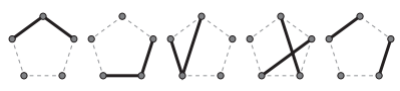
\includegraphics{Figuras/q3c2e1.png}
\end{figure}


Incluindo essas cinco, quantas figuras diferentes podemos fazer desse modo?
\newline\newline
\textcolor{blue}{\bf(4)} (OBMEP 2010) Tio Paulo trouxe cinco presentes diferentes, entre os quais uma boneca, para distribuir
entre suas sobrinhas Ana, Bruna, Cecília e Daniela. De quantos modos ele pode distribuir os presentes entre as sobrinhas de modo que todas ganhem pelo menos um presente e a boneca seja dada para Ana?
\newline\newline
\textcolor{blue}{\bf(5)} (OBMEP 2011) Com os algarismos $1, 4, 6$ e $8$ pode-se formar vários números de três algarismos distintos. Qual é a soma de todos esses números?
\newline\newline
\textcolor{blue}{\bf(6)} (OBMEP 2013) Ana quer fazer duas aulas de natação por semana, uma de manhã e a outra à tarde. A escola de natação tem aulas de segunda a sábado às 9h, 10h e 11h e de segunda a sexta às 17h e 18h. De quantas maneiras distintas Ana pode escolher o seu horário semanal, de modo que ela não tenha suas aulas no mesmo dia nem em dias consecutivos?
\newline\newline
\textcolor{blue}{\bf(7)} (Banco de Questões - OBMEP 2013) Uma minhoca matemática parte do ponto $A$ e chega no ponto $B$ da figura abaixo.

\begin{figure}
    \centering
    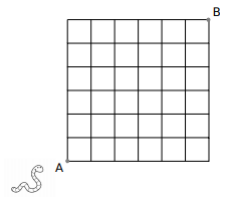
\includegraphics{Figuras/q71c2e1.png}
\end{figure}


Esta minhoca matemática se move sempre sobre as linhas pretas do desenho acima, e nunca passa sobre um lugar no qual ela já esteve anteriormente. Além disso, esta minhoca pode andar para baixo, para cima e para a direita, mas não para a esquerda. Por exemplo, um caminho possível para que a minhoca matemática vá do ponto $A$ ao
ponto $B$ poderia ser:
\begin{figure}[!h]
    \centering
    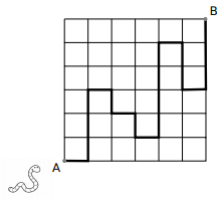
\includegraphics{Figuras/q72c2e1.png}
\end{figure}

\begin{tasks}[counter-format={(tsk[a])},label-width=3.6ex, label-format = {\bfseries}, column-sep = {0pt}](1)
\task[\textcolor{Floresta}{$\negrito{(a)} $}] De quantas maneiras diferentes a minhoca matemática pode ir do ponto $A$ o ponto $B$ através de caminhos contidos nos segmentos mostrados na figura abaixo? (seguindo as regras descritas anteriormente).
\end{tasks}
\begin{figure}[!h]
    \centering
    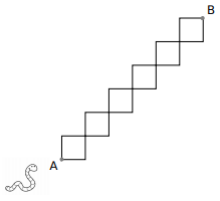
\includegraphics{Figuras/q73c2e1.png}
\end{figure}
\begin{tasks}[counter-format={(tsk[a])},label-width=3.6ex, label-format = {\bfseries}, column-sep = {0pt}](1)
\task[\textcolor{Floresta}{$\negrito{(b)} $}] Qual o número total de maneiras que a minhoca matemática pode ir do ponto $A$ ao
ponto $B?$ (seguindo as regras anteriores, para qualquer caminho, não apenas os do item (a)).
\end{tasks}
\textcolor{blue}{\bf(8)} (OBMEP 2016) Um baralho possui 32 cartas divididas em 4 tipos, cada um com 8 cartas. De quantas formas podemos escolher 6 cartas de modo que todos os quatro tipos de cartas estejam entre elas?
\newline
\newline
\textcolor{blue}{\bf(9)} Um cubo $10 \times 10 \times 10$ é formado por pequenos cubos unitários. Um gafanhoto está no centro $O$ de um dos cubos de canto. Em qualquer instante, ele pode pular para o centro de qualquer cubo que tenha uma face em comum com o cubo onde ele está, desde que este pulo aumente a distância entre o ponto $O$ e a posição atual do gafanhoto. De quantas maneiras o gafanhoto pode chegar ao cubo unitário no canto oposto?
\newline
\newline
\textcolor{blue}{\bf(10)} Quantos números diferentes com $10$ algarismos podem ser escritos usando-se apenas os algarismos $1$ e $2?$
\newline
\newline
\textcolor{blue}{\bf(11)} Uma mangueira tem dez mangas de diferentes tamanhos. De quantas maneiras podemos colher diversas delas?
\newline\newline
\textcolor{blue}{\bf(12)} De quantas maneiras podemos dividir $15$ pessoas em três times de $5$ pessoas?
\newline\newline
\textcolor{blue}{\bf(13)} Para participar de uma loteria esportiva na Rússia, é preciso escolher $6$ dentre $45$ números impressos em um cartão de loteria (todos os cartões são idênticos).
\begin{tasks}[counter-format={(tsk[a])},label-width=3.6ex, label-format = {\bfseries}, column-sep = {0pt}](1)
\task[\textcolor{Floresta}{$\negrito{(a)} $}] De quantas maneiras é possível preencher o cartão da loteria?
\task[\textcolor{Floresta}{$\negrito{(b)} $}] Depois do final da loteria, seus organizadores decidiram contar o número de maneiras de preencher o cartão da loteria de modo que exatamente $3$ dos $6$ números escolhidos estejam entre os $6$ números vencedores. Ajude-os a encontrar a resposta.
\end{tasks} 
\textcolor{blue}{\bf(14) $\varheart$} Seja $n$ um número natural positivo. 
\begin{tasks}[counter-format={(tsk[a])},label-width=3.6ex, label-format = {\bfseries}, column-sep = {0pt}](1)
\task[\textcolor{Floresta}{$\negrito{(a)} $}] Quantas são as soluções inteiras e não negativas de $x_1 + x_2 + x_3 = n,$ se $n = 5?$
\task[\textcolor{Floresta}{$\negrito{(b)} $}] Prove que o número de soluções inteiras e \textbf{não negativas} de $x_1 + x_2 + \ldots + x_k = n$ é $\dbinom{n-1}{k-1}.$
\task[\textcolor{Floresta}{$\negrito{(c)} $}] Prove que o número de soluções inteiras e \textbf{positivas} de $x_1 + x_2 + \ldots + x_k = n$ é $\dbinom{n+k-1}{n}.$
\end{tasks}
%https://artofproblemsolving.com/community/c6h473647p2651848
\textcolor{blue}{\bf(15) $\varheart$} O conjunto $A=\{x_1,x_2,x_3,x_4,x_5,x_6\}$ possui 6 elementos e um conjunto $B= \{y_1,y_2,y_3,\cdots,y_7\}$ possui 7 elementos.
\begin{tasks}[counter-format={(tsk[a])},label-width=3.6ex, label-format = {\bfseries}, column-sep = {0pt}](1)
\task[\textcolor{Floresta}{$\negrito{(a)} $}] Quantas são as funções $f \colon A \to B$?%7^6
\task[\textcolor{Floresta}{$\negrito{(b)} $}] Quantas são as funções injetoras $f \colon A \to B$?%7!


\textbf{Observação:} Este problema é um caso particular do chamado ``\textit{Twelvefold way}'', uma coleção de 12 problemas relacionados a funções e enumerações entre dois conjuntos finitos.
\end{tasks}
\textcolor{blue}{\bf(16) $\varheart$} Um número de dois ou mais algaarismos é chamado de \textit{incrível} se o algarismo das unidades é a soma de todos os demais algarismos. Por exemplo, $1348$ é incrível, pois $1 + 3 + 4 = 8.$
\begin{tasks}[counter-format={(tsk[a])},label-width=3.6ex, label-format = {\bfseries}, column-sep = {0pt}](1)
\task[\textcolor{Floresta}{$\negrito{(a)} $}] Quantos números de $4$ algarismos são incríveis? 
\task[\textcolor{Floresta}{$\negrito{(b)} $}] Quantos são os números incríveis terminados em 3?
\task[\textcolor{Floresta}{$\negrito{(c)} $}] Quantos números incríveis existem?
\end{tasks}
\textcolor{blue}{\bf(17) $\varheart$} Prove o chamado Primeiro Lema de Kaplansky: o número de subconjuntos de $p$ elementos de $\{1, 2, \ldots, n \}$ nos quais não há dois elementos consecutivos é $\dbinom{n-p+1}{p}.$ 
\newline\newline
\textcolor{blue}{\bf(18) $\varheart$} Colocamos vários palitos sobre uma mesa de modo a formar um retângulo $m \times n$, como mostra a figura.
\begin{figure}[!h]
    \centering
    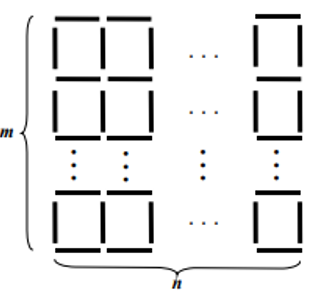
\includegraphics{Figuras/Palitos.png}
\end{figure}

Devemos pintar cada palito de azul, vermelho ou preto de modo que cada um dos quadradinhos da figura seja delimitado por exatamente dois palitos de uma cor e dois de outra cor. 
\begin{tasks}[counter-format={(tsk[a])},label-width=3.6ex, label-format = {\bfseries}, column-sep = {0pt}](1)
\task[\textcolor{Floresta}{$\negrito{(a)} $}] De quantas formas podemos realizar esta pintura?
\task[\textcolor{Floresta}{$\negrito{(b)} $}] Se $m = 7$ e $n = 9,$ mostre que temos $3^{7 + 9} \cdot 2^{7 \cdot 9}$ pinturas. 
\end{tasks}

Exercícios marcados com $\varheart$ são extras.
\end{document}
SetClassGroupBounds("GRH"); 
K := QuadraticField(9);
ClassNumber(K);
Q := PolynomialRing(GF(2), 2);
Q;
K := QuadraticField();
G := GaloisGroup(K);
G;
\begin{CJK}{UTF8}{min}
露の世は 露の世ながら さりながら当時では老人と呼べる50歳代半ばでようやく授かったわが子への愛とその突然死を伝えた「露の世」のくだりは、その日記体句文集「おらが春」のクライマックスとなっています。

5月には数え二歳の誕生を迎えて詠んだ句に、
「這へ笑へ二つになるぞけさからは」と喜びを謳歌したばかり。

それが、翌6月にはもはや草葉の陰へと、その露の朝日に立ちどころに消えるごとく、儚くも身罷ってしまったとは。

人の世は朝露の如く無常なのだと、悔みを述べ慰問するあの人、この人。さは「さりながら」…それは確かにそうなのだけれども。
いかに「あきらめ顔しても、思い切りがたきは、恩愛のきづな也けり。」と、わが心中は耐えきれず切々と泣き崩れるばかり。わが子「さと」女を思う「大切」はやがて「あなた任せ」の境地へと通じていくものでしょう。
\end{CJK}